\section{Farey walls}\label{sec:walls}

The polar coefficients that enter the Rademacher series are sums over matrices of $SL_2(\ZZ)$ attached to Farey intervals, the continued-fraction walls of \cite{CNR21,CV08}. This section collects the elementary facts about them that the estimates need.

\subsection{The walls of a polar term}
Fix $m\ge1$, $\nu\in\frac12\ZZ$ and $\tilde\ell\in\ZZ$ with $0\le\tilde\ell<2m$ and
\[
\tilde D=4m\nu-\tilde\ell^2<0,\qquad t=-\tilde D,\qquad \omega_0=\frac{\tilde\ell}{2m},\qquad \delta=\frac{\sqrt t}{2m}.
\]
Let $\mathcal W(m,\nu,\tilde\ell)$ be the set of $G=\begin{psmallmatrix}p&q\\r&s\end{psmallmatrix}\in SL_2(\ZZ)$ with $r,s\ge1$ and $q/s\le\omega_0<p/r$; for each such $G$ put
\begin{equation}\label{eq:mGnG}
m_G=r^2\nu+p^2m-pr\tilde\ell,\qquad n_G=s^2\nu+q^2m-qs\tilde\ell,\qquad \ell_G=-2rs\nu-2pqm+(ps+qr)\tilde\ell .
\end{equation}
These are the coefficients of the quadratic form $\phi(X,Y)=\nu X^2-\tilde\ell XY+mY^2$ transformed by $G$: $m_G=\phi(r,p)$, $n_G=\phi(s,q)$, and $\ell_G$ is the cross term up to sign.

\begin{lemma}\label{lem:walls}
Let $G\in\mathcal W(m,\nu,\tilde\ell)$ and $U=p/r-\omega_0$, $W=\omega_0-q/s$, so that $U>0$, $W\ge0$ and $U+W=1/rs$.
\begin{enumerate}
\item[(i)] $\ell_G^2-4m_Gn_G=t$.
\item[(ii)] $m_G=mr^2(U^2-\delta^2)$, $n_G=ms^2(W^2-\delta^2)$, $\ell_G=2mrs(UW+\delta^2)>0$, and $m=m_Gs^2+n_Gr^2+\ell_Grs$.
\item[(iii)] $E_G:=m-m_G-n_G-\ell_G=m\big[1-(rU+sW)^2+\delta^2(r-s)^2\big]\ge0$.
\item[(iv)] If $m_G,n_G\ge-1$, put $a=m_G$, $b=n_G$, $S=a+b+2$ and $t_0=m^2+4m$. Then
\begin{equation}\label{eq:t0t}
t_0-t=S(2m-S)+E_G^2+2E_G\ell_G+4(a+1)(b+1),
\end{equation}
so $t\le t_0$; moreover $t_0-t\le2mS$ when $r=s=1$.
\item[(v)] If $m_G,n_G\ge-1$, then $a\le m/s^2$, $b\le m/r^2$ and $r,s\le2m$.
\item[(vi)] If $m_G,n_G\ge-1$ and $rs\ge2$, then $\delta\le\frac14+\frac5{2m}$, that is $\sqrt t\le\frac m2+5$.
\item[(vii)] If $r=s=1$, then $G=\begin{psmallmatrix}1&0\\1&1\end{psmallmatrix}$, $a=\nu+m-\tilde\ell$, $b=\nu$, $\ell_G=m-a-b$, $E_G=0$ and $\tilde\ell=m+b-a$. Conversely every pair $(a,b)$ of integers with $a,b\ge-1$, $k:=m-a-b\ge1$, $t=k^2-4ab>0$ and $-m\le b-a<m$ arises from exactly one polar term with $\nu=b\in\ZZ$ in this way.
\end{enumerate}
\end{lemma}

\begin{proof}
(i) $\phi\circ G$ has the same discriminant as $\phi$. (ii) $\phi(r,p)=r^2\big(\nu-\tilde\ell u+mu^2\big)$ with $u=p/r$, and $\nu-\tilde\ell u+mu^2=m\big((u-\omega_0)^2-\delta^2\big)$ because $\tilde\ell^2-4m\nu=4m^2\delta^2$; similarly for $n_G$. For $\ell_G$ write $\ell_G=2mrs\big[(p/r-\omega_0)(\omega_0-q/s)+\delta^2\big]$, which is \eqref{eq:mGnG} after expanding and using $ps-qr=1$. The last identity follows from $\phi(r,p)s^2+\phi(s,q)r^2+\ell_Grs=m(ps-qr)^2$. (iii) Insert (ii) in the definition and use $U+W=1/rs$; then $rU+sW\le\max(r,s)(U+W)=1/\min(r,s)\le1$. (iv) By (i), $t=\ell_G^2-4ab$ with $\ell_G=m-a-b-E_G=m+2-S-E_G$; expand $t_0-t=m^2+4m-(m+2-S-E_G)^2+4ab$ and use $4ab=4(a+1)(b+1)-4S+4$. For $r=s=1$, $E_G=0$ and $4(a+1)(b+1)\le S^2$. (v) $a=mr^2(U^2-\delta^2)\le mr^2U^2\le m/s^2$, and $b\le m/r^2$ in the same way. Since $t\ge1$, $\delta\ge1/2m$. From $a\ge-1$, $\delta^2\le U^2+1/(mr^2)$, and from $b\ge-1$, $\delta^2\le W^2+1/(ms^2)$. One of $U,W$ is at most $1/(2rs)$; if it is $U$, the first inequality gives $r^2\le4m^2(\frac1{4s^2}+\frac1m)\le m^2+4m$, so $r\le m+1$, and the second with $W\le1/rs$ gives $s^2\le4m^2(1+\frac1m)$, so $s\le2m$. The other case is symmetric. (vi) If $\delta\le\frac14$ there is nothing to prove. Otherwise, from $a\ge-1$, $\delta-U\le1/(mr^2(\delta+U))\le4/(mr^2)$, and from $b\ge-1$, $\delta-W\le4/(ms^2)$. Adding, $2\delta\le\frac1{rs}+\frac4m\big(\frac1{r^2}+\frac1{s^2}\big)\le\frac12+\frac5m$ when $rs\ge2$. (vii) $p-q=1$ and $q\le\omega_0<q+1$ with $0\le\omega_0<1$ force $q=0$, $p=1$. The formulas follow from \eqref{eq:mGnG}. Given $(a,b)$, put $\nu=b$ and $\tilde\ell=m+b-a\in[0,2m)$; then $\tilde D=4mb-(m+b-a)^2=-(k^2-4ab)$.
\end{proof}

\begin{remark}
\begin{figure}[t]
\centering
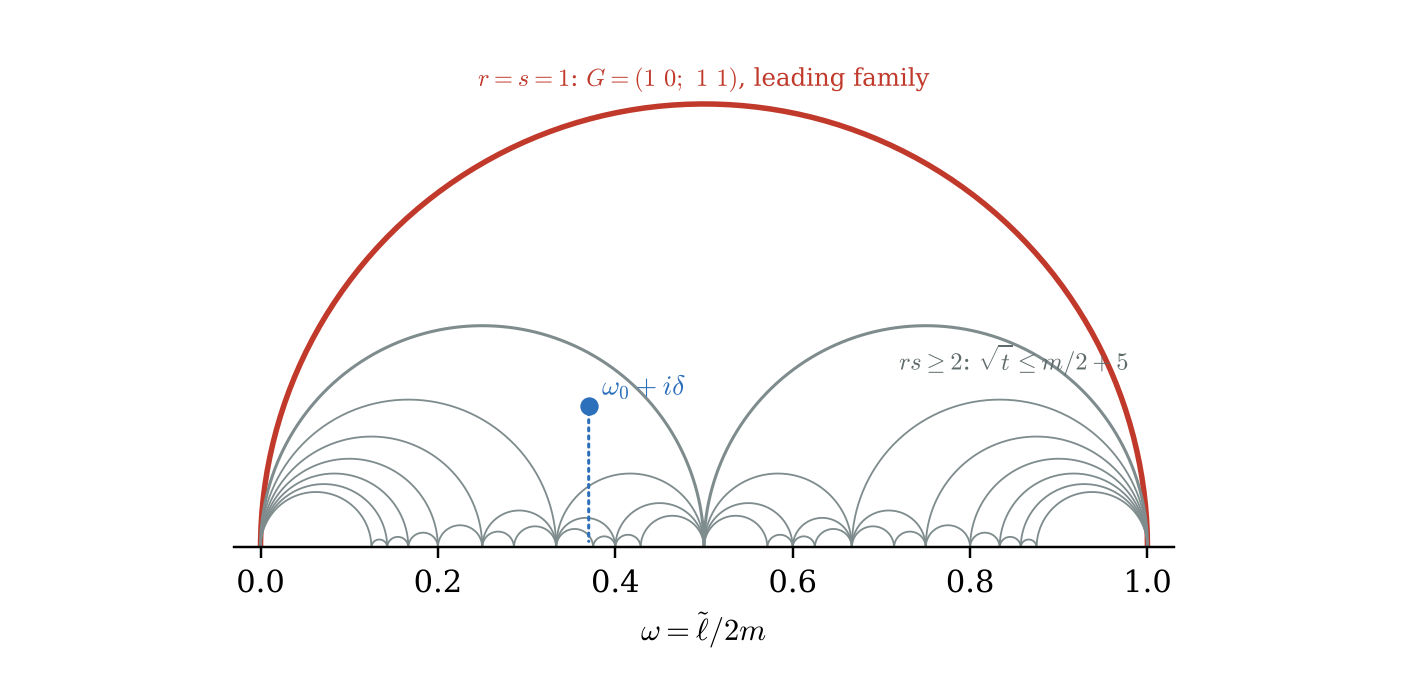
\includegraphics[width=0.86\textwidth]{fig_walls.png}
\caption{The Farey walls of a polar term at the cusp $0$, drawn as geodesics from $q/s$ to $p/r$ in the upper half-plane of $\omega=\tilde\ell/2m$. A matrix $G=\begin{psmallmatrix}p&q\\r&s\end{psmallmatrix}$ contributes to the polar coefficient at $(\tilde\ell,\nu)$ when its geodesic passes over the point $\omega_0+i\delta$ with $\omega_0=\tilde\ell/2m$ and $\delta=\sqrt{-\tilde D}/2m$ (Lemma~\ref{lem:walls}). The outer red geodesic is the leading family $r=s=1$; every other wall lies below height $\frac14+\frac5{2m}$.}\label{fig:wallsfig}
\end{figure}

Lemma~\ref{lem:walls}(iii) is the reason why the leading family dominates: by \eqref{eq:t0t} the walls with $r=s=1$ are exactly those for which $t_0-t$ is as small as the pair $(a,b)$ allows, and by (vi) every other wall has $\sqrt t$ at most about half of $\sqrt{t_0}$. Figure~\ref{fig:wallsfig} shows the geometry.
\end{remark}

\subsection{Polar coefficients}
Let $d_1(k)$, $k\ge-1$, be the coefficients of
\begin{equation}\label{eq:d1}
\frac1{\eta(\tau)^8\eta(2\tau)^8}=\sum_{k\ge-1}d_1(k)\,q^k=q^{-1}+8+52q+256q^2+1122q^3+\cdots,
\end{equation}
so that $d_1(k)=\hat f(k)$ in the notation of \eqref{eq:polar}, and put $d_1(k)=0$ unless $k\ge-1$ is an integer. For a polar term $(\nu,\tilde\ell)$ define
\begin{align}
a_S(\nu,\tilde\ell)&=\frac1{16}\sum_{G\in\mathcal W(m,\nu,\tilde\ell)}\ell_G\,d_1(m_G)\,d_1(n_G)\qquad(\nu\in\ZZ),\label{eq:P0}\\
a_I(\nu,\tilde\ell)&=\sum_{G\in\mathcal W(m,\nu,\tilde\ell)}\ell_G\Big([r\ \text{even}]\,d_1(m_G)\,d_1(2n_G)+[s\ \text{even}]\,d_1(2m_G)\,d_1(n_G)\Big)\qquad(\nu\in\tfrac12\ZZ),\label{eq:Pinf}
\end{align}
and $a_T(\nu,\tilde\ell)=(-1)^{2\nu}a_I(\nu,\tilde\ell)$. The sums are finite by Lemma~\ref{lem:walls}(v). Formula \eqref{eq:P0} is the continued-fraction formula of \cite[(2.43)]{CNR21} for $1/\Phi_{10}$ with the coefficients of $1/\eta^{24}$ replaced by $d_1$ and with no congruence condition on $G$, and \eqref{eq:Pinf} is its parity-restricted form \cite[(4.21)]{CNR21}.\footnote{In \eqref{eq:Pinf} the condition that $r$ or $s$ be even selects the walls that are images of the basic wall under $\Gamma_0(2)$ or its conjugate; the factor $d_1(2n_G)$ vanishes unless $2n_G$ is an integer.}
